\section{Εργαλεία που χρησιμοποιήθηκαν}

Η υλοποίησή αναπτύχθηκε σε γλώσσα Python και χρησιμοποιήθηκαν πληθώρα βιβλιοθηκών όπως η essentia για την εξαγωγή χαρακτηριστικών, η sklearn για την προεπεξεργασία δεδομένων
ενώ στην εκπαίδευση των μοντέλων χρησιμοποιήθηκε η numpy. Χρησιμοποιήθηκε επίσης η  seaborn για την εξαγωγή διαγραμμάτων και την οπτικοποίηση των χαρακτηριστικών. Παράλληλα, σε συνδυασμό με όλες αυτές χρησιμοποιήθηκαν και άλλες βιβλιοθήκες όπως η pandas,  η matplotlib, η multiprocessing, η  οs, η pyaudio κα. Για την εκπαίδευση, δοκιμάστηκαν τα μοντέλα svm, decision trees, multilayer perceptron, Naive bayes και random forest, τα οποία θα αναπτυχθούν στα επόμενα κεφάλαια. Το dataset που χρησιμοποιήθηκε για την εκπαίδευση του μοντέλου είναι το προτινόμενο GTZAN dataset \footnote{http://opihi.cs.uvic.ca/sound/music\_speech.tar.gz}, το οποίο αποτελείται απο 120 αρχεία διάρκειας 30 δευτερολέπτων. Κάθε κλάση (μουσική/φωνή) αποτελείται από 60 αρχεία ενώ δεν υπάρχουν αρχεία που να περιέχουν και τις δύο κλάσεις. Όλα τα δείγματα είναι στα 22050 Hz, Mono 16-bit και σε αρχεία μορφής .wav.

\section{Χαρακτηριστικά}

Για την εξαγωγή των χαρακτηριστικών που φαίνονται στο από τα αρχεία ήχουν του σετ δεδομένων, αρχικά τμηματήσαμε κάθε σήμα αρχείου σε frames με μέγεθος 6144 δείγματα, το οποίο προέκυψε μετά από επαναλαμβανόμενες δοκιμές.
 Έπειτα, τα frames αυτά, παραθυροποιήθηκαν με παράθυρο τύπου Hamming, ίσου μεγέθους. Στη συνέχεια, έγινε η εξαγωγή των χαρακτηριστικών στο πεδίο του χρόνου, καθώς και στο πεδίο της συχνότητας.Παράλληλα, έγινε και η εξαγωγή των συντελεστών MFCC έτσι ώστε να είναι εφικτός ο υπολογισμός της διαμόρφωσης της ενέργειας σήματος στα 4 Ηz. Τα χαρακτηριστικά που εξήχθηκαν, τελικά, είναι τα παρακάτω 27 και θα αναλυθούν στη συνέχεια.

%pinakas me arxikes kai telikes diastaseis xarakthristikwn
% \begin{center}
% \begin{tabular}{ |c |c| }
% \hline
%  cell1 & cell2 & cell3 \\ 
%  cell4 & cell5 & cell6 \\  
%  cell7 & cell8 & cell9    
%  \hline
% \end{tabular}
% \label{table:1}
% \end{center}

\subsection{Zero Crossing Rate - ZCR}

Είναι ο ρυθμός της αλλαγής προσήμου κατά τη διάρκεια του σήματος, δηλαδή ο ρυθμός με τον οποίο το σήμα αλλάζει από θετικό και αρνητικό και αντίστροφα. Σε κάποιο βαθμό, δείχνει την μέση συχνότητα του σήματος ως εξής:
\begin{equation}
\text{ZCR} = \frac{\sum_{m=1}^{N} |sgn ~x(n) - sgn~x(n-1)| }{2N}
\end{equation}

όπου sgn() η συνάρτηση προσήμου και x(m) το διακριτό σήμα ήχου. Στη γενική περίπτωση, το ZCR για την μουσική είναι αρκετά υψιλότερο από ότι στην φωνή.

% \begin{figure}[H]
% \begin{subfigure}{.5\textwidth}
%   \centering
%   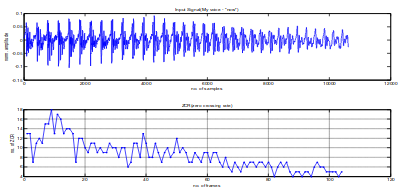
\includegraphics[width=.8\linewidth]{humanvoice.png}
%   \caption{Φωνή}
%   \label{fig:sfig1}
% \end{subfigure}%
% \begin{subfigure}{.5\textwidth}
%   \centering
%   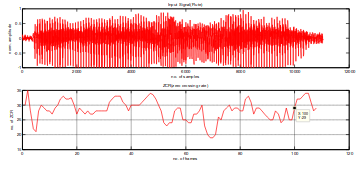
\includegraphics[width=.8\linewidth]{musicinstr.png}
%   \caption{Μουσική}
%   \label{fig:sfig2}
% \end{subfigure}
% \caption{Σήματα φωνής και μουσικής με τα αντίστοιχα ZCR \footnote{Discrimination between Speech and Music signal, Sumit Kumar Banchhor,International Journal of Soft Computing and Engineering (IJSCE)}}
% \label{fig:fig}
% \end{figure}

\subsection{Spectral Centroid - SC}

Το spectral cendroid ή αλλιώς φασματικό κέντρο, όπως αναφέρεται στο \footnote{
Speech and Music Classification and Separation: A Review 
Abdullah I. Al-Shoshan
Department of Computer Science, College of Computer, 
Qassim University, Saudi Arabia },είναι μία μετρική που χρησιμοποιείται ώστε να χαρακτηρίσει ένα φάσμα. Υποδεικνύει πού βρίσκεται το κέντρο του φάσματος. Έχει ισχυρή σύνδεση με την "φωτεινότητα " ενός ήχου δηλαδή με την χροιά. Συνήθως, το κέντρο του φάσματος της φωνής συγκεντρώνεται σε χαμηλές συχνότητες και έπειτα συμπτύσσεται πολύ γήργορα στις υψιλότερες συχνότητες ενώ δεν υπάρχει DC συνιστώσα. Αντίθετα, στην μουσική δεν έχει παρατηρηθεί κάποιο συγκεκριμένο σχήμα του φάσματος. 
\subsection{Roll Off}
 
 Το συγκικριμένο χαρακτηριστικό αναπαριστά την τιμή της συχνότητας, κάτω από την οποία βρίσκεται το 95\% της ενέργειας του σήματος. Όπως προαναφέρθηκε, η ενέργεια του μουσικού σήματος συγκεντρώνεται σε υψηλότερες συχνότητες σε σχέση με το φωνητικό σήμα. Η μαθηματική του έκφραση δίνεται ως:
 \begin{equation}
 \sum_{k<v} X(k) = 0.95 \cdot \sum_{k}X(k)
 \end{equation}
 όπου το X(k) είναι ο διακριτός μετασχηματιμός Fourier (DFT) του x(t),το αριστερό μέρος της παραπάνω εξίσωσης είναι το άθροισμα της ενέργειας κάτω από την συχνότητα v, ενώ το δεξί είναι 95\% της συνολικής ενέργειας του σήματος στο συγκεκριμένο χρονικό frame.

 \subsection{Spectral Flux}

 Το χαρακτηριστικό Spectral Flux ή αλλιώς της φασματικής ροής, όπως αναφέρεται στο 
 cite to oparapanw footnote
 μετράει την φασματική διαφορά ανάμεσα στα frames. Η μουσική έχει μεγαλύτερο ρυθμό διαφοράς ενώ έχει πιο δραστικές αλλαγές ανάμεσα στα frames από ότι η φωνή. Σημειώνεται ότι η μουσική εναλλάσσεται ανάμεσα σε περιόδους μετάβασης και στατικές περιόδους ενώ η φωνή, γενικότερα, έχει έναν πιο σταθερό ρυθμό εναλλαγών. Ως αποτέλεσμα, η τιμή της φασματικής ροής είναι υψηλότερη για την μουσική σε σχέση με την φωνή.

  \subsection{Envelope}

Το envelope είναι ουσιαστικά μία ομαλή καμπύλη που καλύπτει το περίγραμμα ενός ταλαντούμενού σήματος.Εκφράζει, ουσιαστικά, τις χρονικές αλλαγές στο πλάτο του σήματος.Οι αλλαγές αυτές είναι υπεύθυνες για πολλές πτυχές της ακουστικής αντίληψης, συμπεριλαμβανομένου της έντασης, της χροιάς, της οξύτητας και τις χωρικής ακουστότητας.


\subsection{Flatness}

To flatness ή αλλιώς επιπεδότητα του ήχου, είναι μία μετρική η οποία χρησιμοποιείται στην ανάλυση ψηφιακών σημάτων για να χαρακτηρίσει το φάσμα ενός ηχητικού σήματος. Συνήθως μετριέται σε decibels (DB), και αποτελεί έναν τρόπο να ποσοτικοποιήσει το πόσο κοντά είναι ένας ήχος σε θόρυβο και πόσο σε τονικότητα.  \footnote{https://en.wikipedia.org/wiki/Spectral\_flatness} Η αναφορά στην τονικότητα γίνεται με την έννοια του αρίθμού των κορυφών σε ένα φάσμα συχνοτήτων που θα υπήρχαν λόγω των πολλαπλών ημιτόνων σε αντίθεση με το επίπεδο φάσμα του λευκού θορύβου. Τα μουσικά σήματα, τείνουν να αποτελούνται από πολλαπλούς τόνους, ο καθένας με την δική του κατανομή αρμονικών ενώ στην φωνή δεν εμφανίζεται αυτό.


\subsection{Perceptual attack time}

Αυτό το χαρακτηριστικό αναφέρεται στην χρονική διάρκεια ανάμεσα στη χρονική στιγμή που το σήμα γίνεται ακουστικά αντιληπτό μέχρι τη χρονική στιγμή που φτάνει την μέγιστη έντασή του. 

\subsection{Sound Decay}

Η προοδευτική μείωση του πλάτους ενός σήματος με την πάροδο του χρόνου. Αυτή η φάση ξεκινάει μόλις το perceptual attack time φτάσει στο μέγιστό του. Σε αυτήν την φάση το πλάτος του σήματος μειώνεται μέχρι να φτάσει σε ένα συγκεκριμένο πλάτος στο οποίο διατηρείται μέχρι να αρχίσει να σβήνει.


\subsection{Spectral Complexity}
 
 To spectral complexity ή αλλιώς η φασματική πολυπλοκότητα, βασίζεται στον αριθμό των κορυφών του φάσματος του σήματος.

\subsection{Mel Frequency Cepstral Coefficient - MFCC }

Στην επεξεργασία ήχου, το cepstrum συχνοτήτων Mel (Μel frequency cepstrum - MFC)
είναι μια αναπαράσταση του βραχυπρόθεσμου φάσματος έντασης ενός ήχου, βασισμένου σε έναν γραμμικό μετασχηματισμό συνημιτόνου του λογαριθμισμένου φάσματος έντασης σε μια μη γραμμική κλίμακα της συχνότητας (μη γραμμικής κλίμακας Mel).  Οι συντελεστές του cepstrum συχνότητας Μελ (MFCCs – Mel Frequency Cepstrum Coefficients) είναι οι συντελεστές εκείνοι που αποτελούν στο σύνολο τους το φάσμα MFC.


\subsection{4Hz Energy Modulation}

Τα φωνητικά σήματα έχουν χαρακτηριστικό μέγιστο στη διαμόρφωση ενέργειας γύρω στα 4Hz του ρυθμού συλλαβών. Για να μοντελοποιηθεί αυτή η ιδιότητα ακολουθείται η παρακάτω διαδικασία:\footnote{https://www.irit.fr/recherches/SAMOVA/FeaturesExtraction.htm\#me4hz} Το σήμα τμηματοποιείται σε frames και εξάγονται οι Mel Frequency Spectrum Coefficients \footnote{https://en.wikipedia.org/wiki/Mel-frequency\_cepstrum} και υπολογίζεται η ενέργεια σε 40 κανάλια αντίληψης. Αυτή η ενέργεια έπειτα φιλτράρεται με ένα ζωνοδιαβατό φίλτρο, κεντραρισμένο στα 4Hz. Η ενέργεια αθροίζεται για όλα τα κανάλια, και κανονικοποιείται με βάση το μέσο του κάθε frame. Η διαμόρφωση δίνεται από τον υπολογισμό της μεταβλητότητας της φιλτραρισμένης ενέργειας σε dB σε ένα δευτερόλεπτο του σήματος. Η φωνή περιέχει περισσότερη διαμόρφωση από την μουσική.
%Leptomeries gia tin diki mas ulopoihsh, epilogh timwn ktl


\par Παρακάτω φαίνονται ενδεικτικά κάποια από τα παραπάνω χαρακτηριστικά και το πόσο αποτελεσματικά είναι στον διαχωρισμό:

\begin{figure}[H]
\centering
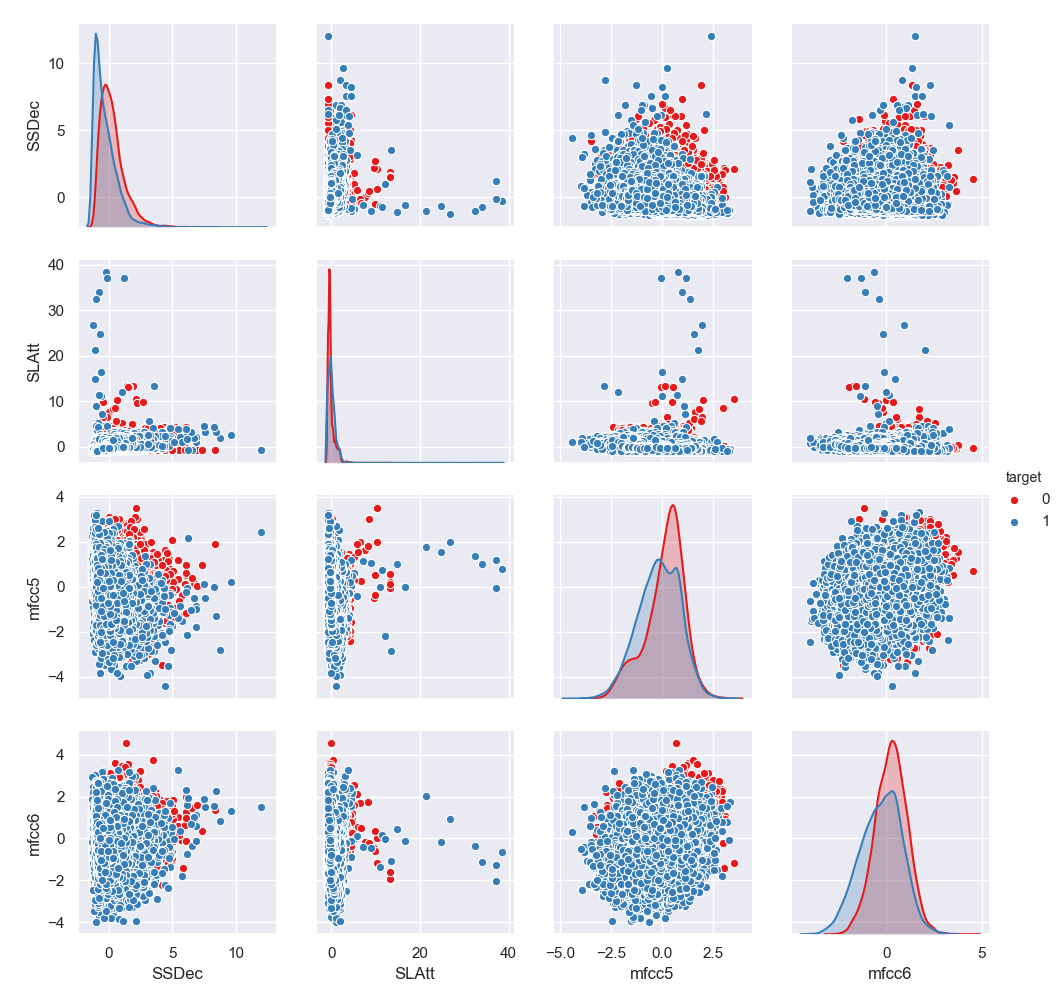
\includegraphics[width=0.7\textwidth]{res/figure_1.png}
\end{figure}
\begin{figure}[h]
\centering
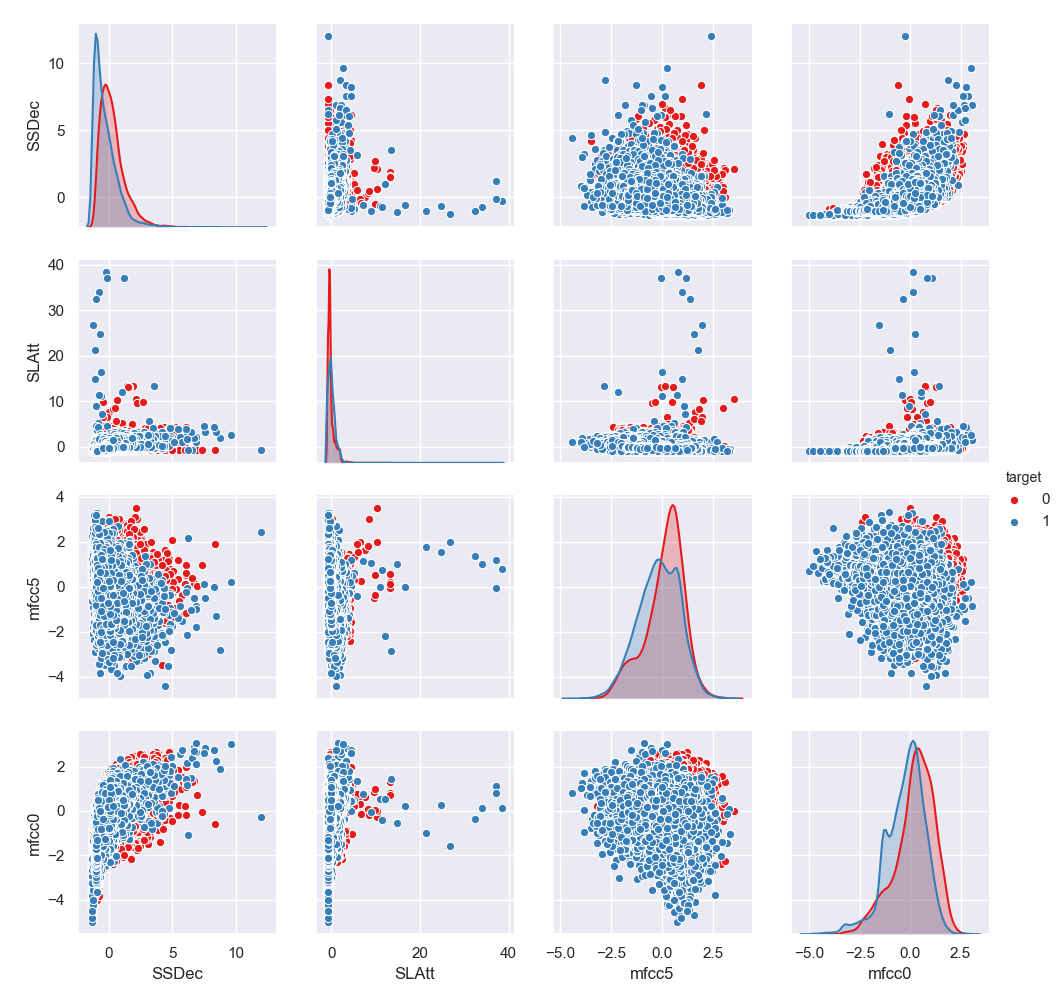
\includegraphics[width=0.7\textwidth]{res/figure_2.png}
\caption{Αποτελεσματικότητα χαρακτηριστικών στον διαχωρισμό των κλάσεων}
\end{figure}


\section{Προεπεξεργασία δεδομένων}
Για την προεπεξεργασία των δεδομένων, δοκιμάστηκαν διάφορες τεχνικές έτσι ώστε να βρεθεί ο βέλτιστος συνδυασμός μεθόδων. Οι τρόποι που δοκιμάστηκαν είναι οι κλιμακοποίηση, κανονικοποίηση, VarianceThreshold, PercentileSelection και ο συνδυασμός τους μαζί με την αλλαγή κάποιων παραμέτρων. Τα αποτελέσματα παρουσιάζονται στον πίνακα \ref{table:tab}
Στην κλιμακοποίηση όλα τα χαρακτηριστικά έχουν μέσο 0 και απόκλιση ίση με 1 ενώ στην κανονικοποίηση, μετατρέπονται οι τιμές τους ώστε να ανήκουν στο εύρος [0,1].  Στο VarianceThreshold και PercentileSelection, που είναι συναρτήσεις της βιβλιοθήκης feature\_selection της sklearn, γίνεται μείωση χαρακτηριστικών. Στο VarianceThreshold, η μείωση γίνεται με όρους διακύμανσης, δηλαδή
αφαιρεί όλα τα χαρακτηριστικά των οποίων η διακύμανση δεν ξεπερνά κάποιο κατώφλι, ενώ η PercentileSelection καταργεί όλα τα ποσοστά των χαρακτηριστικών, εκτός από αυτά με καθορισμένο από το χρήστη καλύτερη ποσοστιαία κατάταξη . % removes all but a user-specified highest scoring percentage of features -> better translate?

\begin{table}[H]
\begin{tabular}{|l|l|l|}
\hline
\textbf{Μέθοδος}       & \textbf{Τρόπος προεπεξεργασίας}                                             & \textbf{Ακρίβεια}            \\ \hline
                       & Χωρίς προεπεξεργασία                                                        & 0.49                         \\ \cline{2-3} 
                       & Κλιμακοποίηση                                                               & 0.89                         \\ \cline{2-3} 
                       & Κανονικοποίηση                                                              & 0.49                         \\ \cline{2-3} 
                       & Κλιμακοποίηση + μετά κανονικοποίηση                                         & 0.78                         \\ \cline{2-3} 
                       & VarianceThreshold + κλιμακοποίηση                                           & 0.88                         \\ \cline{2-3} 
                       & PercentileSelection + κλιμακοποίηση                                         & 0.81                         \\ \cline{2-3} 
                       & VarianceThreshold,  κλιμακοποίηση + gamma=scale                             & 0.88                         \\ \cline{2-3} 
                       & VarianceThreshold,  κλιμακοποίηση + sigmoid kernel                          & 0.58                         \\ \cline{2-3} 
\multirow{-9}{*}{SVM}  & VarianceThreshold,  κλιμακοποίηση + poly kernel dgr                         & 0.84                         \\ \hline
Decision Tree          & VarianceThreshold + κλιμακοποίηση                                           & 0.75                         \\ \hline
Multi-Layer Perceptron & VarianceThreshold, κλιμακοποίηση + rndState = 2                             & 0.86                         \\ \hline
Naive Bayes            & VarianceThreshold + κλιμακοποίηση                                           & 0.65                         \\ \hline
\end{tabular}
\caption{Τρόποι προεπεξεργασίας για διάφορα μοντέλα}
\label{table:tab}
\end{table}

Εν τέλει, αποφασίστηκε να χρησιμοποιηθεί μόνο η κλιμακοποίηση καθώς το κέρδος σε ταχύτητα των παραπάνω τρόπων μείωσης μεταβλητών δεν ήταν αρκετό συγκριτικά με την μείωση της ακρίβειας ώστε να παραμείνουν στην υλοποίηση. Βοήθησαν παρ'όλα αυτά στον προσδιορισμό των χαρακτηριστικών που είναι κάπως καλύτερα από τα άλλα.



Στη συνεχεια, για να γίνει κατανοητό εάν τα χαρακτηριστικά που είναι καλύτερα, είναι ικανά να δώσουν μεγάλο ποσοστό ακρίβειας στο μοντέλο, απομονώθηκαν όλα και ελέχθηκαν ένα ένα. 
Tα αποτελέσματα έδειξαν ότι, τελικά, κανένα χαρακτηριστικό από μόνο του δεν είναι ικανό να δώσει ικανοποιητικό ποσοστό ακρίβειας0. Ακόμα και αν πάρουμε το καλύτερο σε όρους ακρίβειας και το δοκιμάσουμε σε συνδυασμό με τα επόμενα καλύτερα, φαίνεται ότι η ακρίβεια αυξάνεται λίγο αλλά όχι αρκετά.  
Τέλος, αν επαναληφθεί ακόμα μία φορά η διαδικασία, φαίνεται ότι έχουμε και πάλι μια μικρή αύξηση στην ακρίβεια, η οποία όμως είναι αρκετά μακρυά από την ακρίβεια που επιτυγχάνεται εν τέλει. 

\begin{table}[H]
\begin{tabular}{|l|l|l|l|}
\hline
\textbf{Accuracy}       & \textbf{Individually}       & \textbf{with best 1}       & \textbf{with best 2}       \\\hline
4Hz Mod                 & 0.58                        & 0.66                       & 0.73                       \\\hline
Flat                    & 0.63                        & 0.71                       & 0.75                       \\\hline
HFC                     & 0.58                        & 0.65                       & 0.72                       \\\hline
LAtt                    & 0.62                        & 0.71                       & 0.75                       \\\hline
SC                      & 0.59                        & 0.66                       & 0.73                       \\\hline
Scomp                   & 0.57                        & 0.66                       & 0.73                       \\\hline
SDec                    & 0.63                        & 0.65                       & 0.72                       \\\hline
SEFlat                  & 0.51                        & 0.65                       & 0.72                       \\\hline
SF                      & 0.55                        & 0.69                       & 0.75                       \\\hline
SFlat                   & 0.57                        & 0.66                       & 0.72                       \\\hline
SLAtt                   & 0.63                        & 0.71                       & 0.74                       \\\hline
SR                      & 0.60                        & 0.66                       & 0.72                       \\\hline
SSDec                   & \textbf{0.65}               & -                          & -                          \\\hline
ZCR                     & 0.58                        & 0.65                       & 0.72                       \\\hline
mfcc0                   & 0.61                        & 0.66                       & 0.73                       \\\hline
mfcc1                   & 0.58                        & 0.67                       & 0.73                       \\\hline
mfcc2                   & 0.52                        & 0.66                       & 0.73                       \\\hline
mfcc3                   & 0.56                        & 0.69                       & 0.76                       \\\hline
mfcc4                   & 0.54                        & 0.67                       & 0.74                       \\\hline
mfcc5                   & 0.57                        & 0.70                       & 0.75                       \\\hline
mfcc6                   & 0.61                        & \textbf{0.72}              & -                          \\\hline
mfcc7                   & 0.57                        & 0.68                       & 0.75                       \\\hline
mfcc8                   & 0.55                        & 0.67                       & 0.74                       \\\hline
mfcc9                   & 0.54                        & 0.67                       & 0.73                       \\\hline
mfcc10                  & 0.54                        & 0.65                       & 0.73                       \\\hline
mfcc11                  & 0.51                        & 0.66                       & 0.73                       \\\hline
mfcc12                  & 0.54                        & 0.67                       & 0.73                       \\\hline
\end{tabular}
\caption{Ακρίβεια μεμονωμένων χαρακτηριστικών και συνδυασμών τους}
\end{table}
%Διαγραμμα features-απόδοσης;
Άρα, είναι προφανές ότι δεν είναι κάποιο συγκεκριμένο χαρακτηριστικό το οποίο ευθύνεται για το μεγαλύτερο ποσοστό της ακρίβειας του μοντέλου αλλά ο συνδυασμός τους.









